\documentclass[]{elsarticle} %review=doublespace preprint=single 5p=2 column
%%% Begin My package additions %%%%%%%%%%%%%%%%%%%
\usepackage[hyphens]{url}

  \journal{Transport Findings} % Sets Journal name


\usepackage{lineno} % add
\providecommand{\tightlist}{%
  \setlength{\itemsep}{0pt}\setlength{\parskip}{0pt}}

\usepackage{graphicx}
\usepackage{booktabs} % book-quality tables
%%%%%%%%%%%%%%%% end my additions to header

\usepackage[T1]{fontenc}
\usepackage{lmodern}
\usepackage{amssymb,amsmath}
\usepackage{ifxetex,ifluatex}
\usepackage{fixltx2e} % provides \textsubscript
% use upquote if available, for straight quotes in verbatim environments
\IfFileExists{upquote.sty}{\usepackage{upquote}}{}
\ifnum 0\ifxetex 1\fi\ifluatex 1\fi=0 % if pdftex
  \usepackage[utf8]{inputenc}
\else % if luatex or xelatex
  \usepackage{fontspec}
  \ifxetex
    \usepackage{xltxtra,xunicode}
  \fi
  \defaultfontfeatures{Mapping=tex-text,Scale=MatchLowercase}
  \newcommand{\euro}{€}
\fi
% use microtype if available
\IfFileExists{microtype.sty}{\usepackage{microtype}}{}
\bibliographystyle{elsarticle-harv}
\usepackage{graphicx}
% We will generate all images so they have a width \maxwidth. This means
% that they will get their normal width if they fit onto the page, but
% are scaled down if they would overflow the margins.
\makeatletter
\def\maxwidth{\ifdim\Gin@nat@width>\linewidth\linewidth
\else\Gin@nat@width\fi}
\makeatother
\let\Oldincludegraphics\includegraphics
\renewcommand{\includegraphics}[1]{\Oldincludegraphics[width=\maxwidth]{#1}}
\ifxetex
  \usepackage[setpagesize=false, % page size defined by xetex
              unicode=false, % unicode breaks when used with xetex
              xetex]{hyperref}
\else
  \usepackage[unicode=true]{hyperref}
\fi
\hypersetup{breaklinks=true,
            bookmarks=true,
            pdfauthor={},
            pdftitle={Using Google Community Mobility Reports to investigate the incidence of COVID-19 in the United States},
            colorlinks=false,
            urlcolor=blue,
            linkcolor=magenta,
            pdfborder={0 0 0}}
\urlstyle{same}  % don't use monospace font for urls

\setcounter{secnumdepth}{0}
% Pandoc toggle for numbering sections (defaults to be off)
\setcounter{secnumdepth}{0}


% Pandoc header
\usepackage{booktabs}
\usepackage{longtable}
\usepackage{array}
\usepackage{multirow}
\usepackage{wrapfig}
\usepackage{float}
\usepackage{colortbl}
\usepackage{pdflscape}
\usepackage{tabu}
\usepackage{threeparttable}
\usepackage{threeparttablex}
\usepackage[normalem]{ulem}
\usepackage{makecell}
\usepackage{xcolor}



\begin{document}
\begin{frontmatter}

  \title{Using Google Community Mobility Reports to investigate the incidence of
COVID-19 in the United States}
    \author[McMaster University]{Antonio Paez\corref{1}}
   \ead{paezha@mcmaster.ca} 
      \address[McMaster University]{School of Geography and Earth Sciences, McMaster University, Hamilton,
ON, L8S 4K1, Canada}
      \cortext[1]{Corresponding Author}
  
  \begin{abstract}
  In 2020 Google released a set of Community Mobility Reports (GCMR).
  These reports are based on the company's location-tracking capabilities
  and measure changes in mobility with respect to a baseline. This novel
  source of data offers an opportunity to investigate potential
  correlations between mobility and incidence of COVID-19. Using data from
  the New York Times on COVID-19 cases and GCMR, this paper presents an
  analysis of mobility levels and incidence of COVID-19 by state in the
  US. The results provide insights about the utility and interpretability
  of GCMR for COVID-19 research and decision-making.
  \end{abstract}
  
 \end{frontmatter}

\hypertarget{research-questions-and-hypotheses}{%
\section{Research Questions and
Hypotheses}\label{research-questions-and-hypotheses}}

The main policy tool to control the spread of the COVID-19 pandemic has
been restrictions to non-essential travel in the form of stay-at-home
orders. In the United States, such orders have been implemented on a
state-by-state basis with considerable variations in compliance.
Concurrently, numerous initiatives have been developed to track the
progress and the impact of the pandemic. As a result, there are new
sources of data such as the recently-released Google Community Mobility
Reports (GCMR)\footnote{https://www.google.com/covid19/mobility/}, as
well as The New York Times repository of COVID-19
data\footnote{https://github.com/nytimes/covid-19-data}. These two open
data sets offer novel opportunities to investigate in quasi-real time
the relationship between mobility patterns and transmission of COVID-19.

This paper investigates the potential of Google Community Mobility
Reports to asses the impact of mobility on the incidence of COVID-19.
The following questions are posed:

\begin{itemize}
\tightlist
\item
  Do changes in mobility according to GCMR correlate with the incidence
  of COVID-19?
\item
  And if so, what do we learn about mobility and the spread of the
  disease?
\end{itemize}

This paper is a reproducible research document. The source is an
\texttt{R} markdown file available in a public
repository\footnote{See folder Covid-19-Google-CMR-US in \url{https://github.com/paezha/Google-Mobility-Reports-and-COVID-19-US/}}.

\hypertarget{methods-and-data}{%
\section{Methods and Data}\label{methods-and-data}}

GCMR use aggregated and anonymized data to chart changes in mobility
with respect to different classes of places (see Table
\ref{tab:descriptive-statistics}). Mobility indicators are calculated
based on the frequency and length of visits to places. The reports give
percentage change from a baseline level, which corresponds to the median
value of mobility of identical days of the week during the period
between January 3 and Feb 6, 2020. Covid-19 data is compiled by The New
York Times based on reports from state and local health agencies.

\begin{table}[H]

\caption{\label{tab:descriptive-statistics}\label{tab:descriptive-statistics}Descriptive statistics of the data set}
\centering
\resizebox{\linewidth}{!}{
\fontsize{7}{9}\selectfont
\begin{tabular}[t]{l>{\raggedright\arraybackslash}p{12em}llll}
\toprule
Variable & Definition & min & median & max & sd\\
\midrule
\rowcolor{gray!6}  Incidence & Total cases of COVID-19 divided by population (in 100,000s) & 0.01 & 56.87 & 1710.06 & 229.76\\
date & Date & 2020-02-27 & 2020-04-08 & 2020-05-09 & \\
\rowcolor{gray!6}  retail & Mobility trends for places like restaurants, cafes, shopping centers, theme parks, museums, libraries, and movie theaters & 0.34 & 0.66 & 1.16 & 0.2\\
groceries & Mobility trends for places like grocery markets, food warehouses, farmers markets, specialty food shops, drug stores, and pharmacies & 0.66 & 0.93 & 1.26 & 0.12\\
\rowcolor{gray!6}  parks & Mobility trends for places like local parks, national parks, public beaches, marinas, dog parks, plazas, and public gardens & 0.36 & 1.15 & 2.28 & 0.29\\
\addlinespace
transit & Mobility trends for places like public transport hubs such as subway, bus, and train stations & 0.24 & 0.7 & 1.14 & 0.22\\
\rowcolor{gray!6}  work & Mobility trends for places of work & 0.34 & 0.62 & 1.05 & 0.18\\
residential & Mobility trends for places of residence & 0.98 & 1.14 & 1.27 & 0.07\\
\bottomrule
\multicolumn{6}{l}{\textit{Note: }}\\
\multicolumn{6}{l}{All mobility indicators are lagged 11-day moving averages}\\
\end{tabular}}
\end{table}

For analysis, all mobility indicators are centered so that the value of
1 is the baseline mobility, and a 0.01 deviation corresponds to a 1\%
change. The incubation time of the disease is between 2 and 12 days
(95\% interval; see Lauer et al., 2020). Given this, it is to be
expected that any changes in mobility will have a lagged effect on the
discovery of new cases. For this reason, lagged moving averages of the
mobility indicators are calculated. Furthermore, it is possible that
mobility and reports of new cases of COVID-19 are endogenous, if the
public adjust their mobility according to reports of the incidence.
Therefore, in addition to being consistent with an incubation period,
use of lagged indicators also helps to break this potential endogeneity.

The lagged indicators are calculated as the mean of the mobility
indicator using the values from date-minus-12-days to date-minus-2-days.
Furthermore, using the cumulative number of reported COVID-19 cases, the
incidence is calculated after dividing by the population of the state
(in 100,000s). This variable (log-transformed) is paired with the
corresponding lagged moving average of the mobility indicators. The
log-transformation is useful to avoid negative values of incidence when
making predictions. Table \ref{tab:descriptive-statistics} shows the
descriptive statistics of the data set. Analysis is based on correlation
analysis, multivariate regression, and data visualization.

\hypertarget{findings}{%
\section{Findings}\label{findings}}

Table \ref{tab:correlation-analysis-log-incidence} shows that the
mobility indicators are highly correlated with each other. Two variables
are selected for multivariate analysis: parks- and work-related
mobility. Work has a high correlation with the outcome variable, and its
correlation with parks is relatively weak, which increases the
information content of the two variables in multivariate analysis.
Furthermore, parks- and work-related mobility represent two dimensions
of out-of-home activities: mandatory and discretionary travel.

\begin{table}

\caption{\label{tab:check-correlations-log-incidence}\label{tab:correlation-analysis-log-incidence}Simple correlation between log(incidence) and the mobility indicators}
\centering
\resizebox{\linewidth}{!}{
\fontsize{7}{9}\selectfont
\begin{tabular}[t]{lrrrrrrr}
\toprule
  & log\_incidence & retail & groceries & parks & transit & work & residential\\
\midrule
\rowcolor{gray!6}  log\_incidence & 1.00 & -0.86 & -0.73 & -0.20 & -0.82 & -0.91 & 0.89\\
retail & -0.86 & 1.00 & 0.88 & 0.38 & 0.91 & 0.96 & -0.98\\
\rowcolor{gray!6}  groceries & -0.73 & 0.88 & 1.00 & 0.41 & 0.88 & 0.87 & -0.88\\
parks & -0.20 & 0.38 & 0.41 & 1.00 & 0.46 & 0.33 & -0.36\\
\rowcolor{gray!6}  transit & -0.82 & 0.91 & 0.88 & 0.46 & 1.00 & 0.92 & -0.93\\
\addlinespace
work & -0.91 & 0.96 & 0.87 & 0.33 & 0.92 & 1.00 & -0.98\\
\rowcolor{gray!6}  residential & 0.89 & -0.98 & -0.88 & -0.36 & -0.93 & -0.98 & 1.00\\
\bottomrule
\multicolumn{8}{l}{\textit{Note: }}\\
\multicolumn{8}{l}{All mobility indicators are lagged 11-day moving averages}\\
\end{tabular}}
\end{table}

A regression model is estimated with the log of incidence as the
dependent variable. The covariates enter the regression in the form of a
second order polynomial expansion. In addition, the date (centered on
April 5) is introduced to account for the temporal trend of the
pandemic. Finally, an indicator variable for the state of New York is
used to distinguish the unusually high incidence of the disease there.
The results of the model are shown in Table
\ref{tab:model-results-log-incidence}. The model provides a good fit to
the data and all variables reported are significant at \(p<0.10\) or
better.

There is an overall temporal trend that indicates a growing incidence
over time, but at a decelerating rate (see negative sign of date\^{}2).
Mobility related to parks and to work are both associated with higher
incidence of COVID-19, however, the effect of parks-related mobility
grows non-linearly (see positive sign of quadratic term), whereas the
effect of work-related mobility grows at a decreasing rate (see negative
sign of quadratic term). Furthermore, the negative sign for the
interaction of these two mobility indicators captures the trade-offs
between these two forms of mobility and their impact on incidence. The
influence of parks-related mobility was relatively weak early in the
pandemic (negative sign of the parks x date term) but has become more
important over time (positive sign of the parks x date\^{}2 term). The
opposite happens with work-related mobility, the importance of which has
declined over time (negative sign of work x date\^{}2 term), but whose
impact has declined over time (negative sign of work x date\^{}2 term).
As seen in the table, incidence of COVID-19 in New York is consistently
higher.

\begin{table}[H]

\caption{\label{tab:model-results-log-incidence}\label{tab:model-results}Results of estimating regression model. Dependent variable is log(Incidence).}
\centering
\fontsize{7}{9}\selectfont
\begin{tabular}[t]{lcc}
\toprule
Variable & Coefficient Estimate & p-value\\
\midrule
\rowcolor{gray!6}  date & 0.1618 & <0.001\\
date\textasciicircum{}2 & -0.0008 & 0.0093\\
\rowcolor{gray!6}  parks\textasciicircum{}2 & 0.2518 & 0.0562\\
parks & 4.1307 & <0.001\\
\rowcolor{gray!6}  parks x work & -8.1480 & <0.001\\
\addlinespace
work & 9.4568 & <0.001\\
\rowcolor{gray!6}  work\textasciicircum{}2 & -3.4421 & <0.001\\
parks x date & -0.0948 & <0.001\\
\rowcolor{gray!6}  parks x date\textasciicircum{}2 & 0.0036 & <0.001\\
work x date\textasciicircum{}2 & -0.0058 & <0.001\\
\addlinespace
\rowcolor{gray!6}  NY & 1.8627 & <0.001\\
\bottomrule
\multicolumn{3}{l}{\textit{Note: }}\\
\multicolumn{3}{l}{Coefficient of Determination $R^2$= 0.972}\\
\multicolumn{3}{l}{Adjusted Coefficient of Determination $R^2$= 0.972}\\
\multicolumn{3}{l}{Standard Error $\sigma$= 0.689}\\
\end{tabular}
\end{table}

Visualization is the most effective way to understand the trend
according to the mobility indicators and date. Figure
\ref{fig:prediction-plots} shows the prediction surfaces on four
different dates at intervals of 15 days: March 21, when the first states
began implementing stay-at-home orders; then April 5, two weeks into the
lockdown; this is followed by April 20, at a time when some states
started to consider relaxing stay-at-home orders; and finally May 5,
when some states were reopening and/or letting stay-at-home orders
lapse.

On March 21 there were still only minor departures from the baseline
level of mobility (recall that these are temporally lagged); the
prediction surface at this point is relatively flat. This changes by
April 5, when work-based mobility has declined substantially. Although
every state registers lower work-based mobility, there are large
variations in parks-based mobility, with some states seeing increases of
up to 60\% for this class of mobility. By May 5, park-related mobility
in some states had increased to 200\% of the baseline.

The prediction surfaces are hyperbolic paraboloids on any given date,
and in general indicate an expectation of higher incidences as either
class of mobility increases, but with a progressively steeper trend for
park-based mobility over time. On the last date examined, May 5, the
trend becomes more steep for park-based mobility, even as this indicator
continues to display large variations from the baseline in both
directions. The white dashed lines in the plots are the folds of the
saddles, and represent, for each date, the combination of parks- and
work-related mobility levels that tended to minimize the incidence.

\begin{figure}
\centering
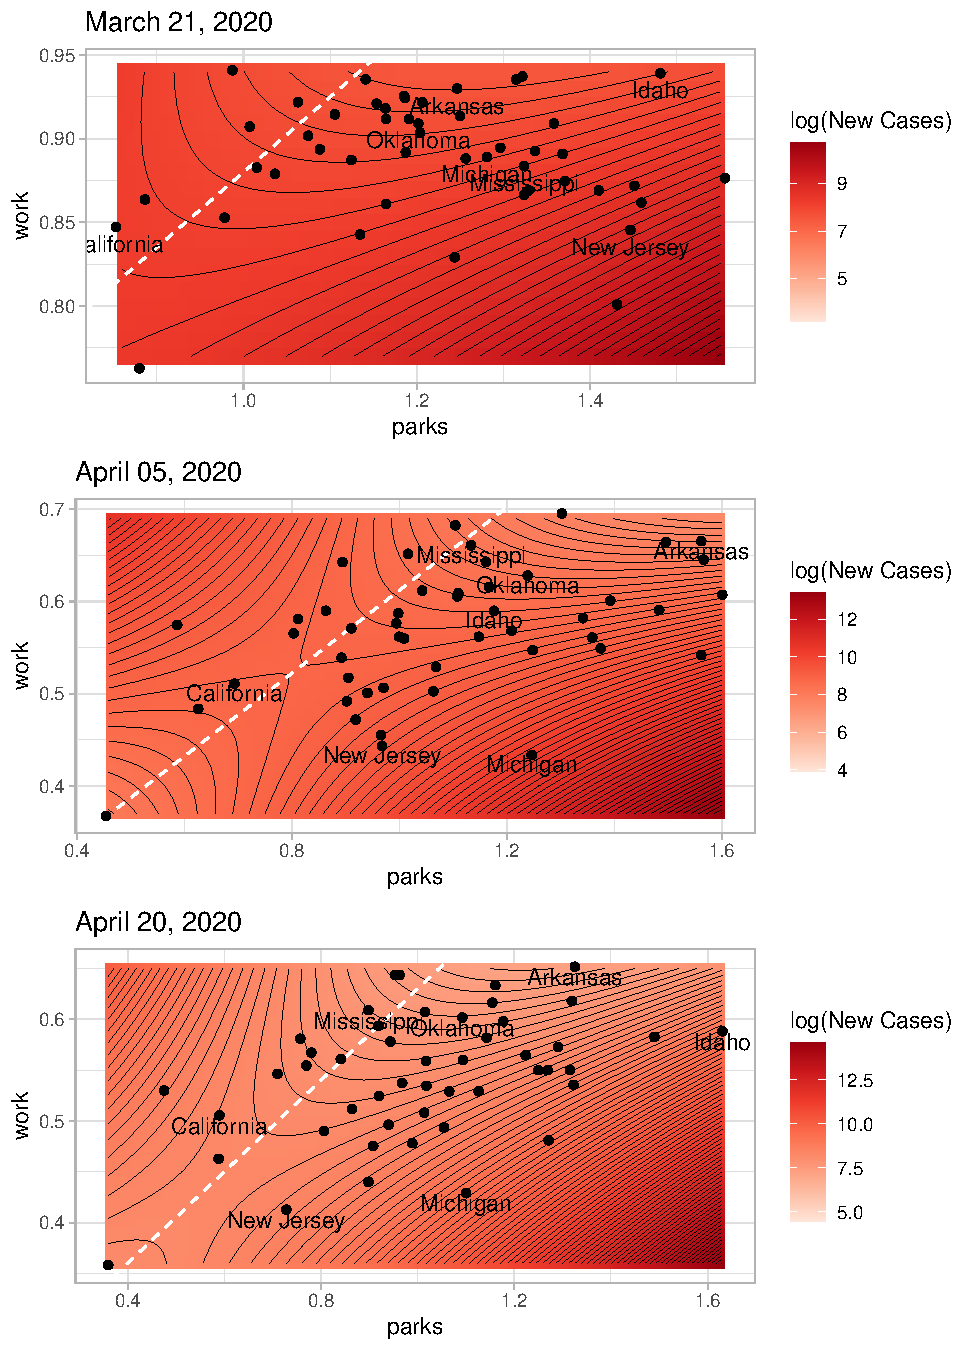
\includegraphics{Covid-19-Google-CMR-US_files/figure-latex/prediction-plots-1.pdf}
\caption{\label{fig:prediction-plots}Prediction surfaces at three points
during the pandemic according to the model; the dots are a scatterplot
of the parks- and work-related mobility indicators of the states on that
date; the white dashed line is the fold of the saddle.}
\end{figure}

The results suggest that over time the benefits of reduced work-related
mobility can be easily offset by parks-related mobility. For example,
California has consistently registered lower levels of parks-related
mobility whereas Idaho has had high levels of this kind of mobility
throughout the pandemic. The incidence of COVID-19 grew in the
intervening period; however, between March 21 and May 5 growth in
incidence in California was 876.42\% whereas Idaho's growth in incidence
over the same period was 2519.05\%.

These results suggest the potential of GCMR to investigate the potential
effects of mobility on the incidence of COVID-19. In particular, growth
appears to be more strongly driven by parks-related mobility. In terms
of the use of these mobility indicators, there are some limitations that
must be acknowledged. The baseline level is not defined in a metric that
is amenable to policy development (e.g., person-km travelled). Without a
clearer understanding of the absolute levels of these variables, these
indicators are useful for inference and perhaps short-term forecasting,
but their potential for applied policy analysis appears to be more
limited.

\hypertarget{references}{%
\section*{References}\label{references}}
\addcontentsline{toc}{section}{References}

\hypertarget{refs}{}
\leavevmode\hypertarget{ref-Lauer2020incubation}{}%
Lauer, S.A., Grantz, K.H., Bi, Q., Jones, F.K., Zheng, Q., Meredith,
H.R., Azman, A.S., Reich, N.G., Lessler, J., 2020. The incubation period
of coronavirus disease 2019 (covid-19) from publicly reported confirmed
cases: Estimation and application. Annals of Internal Medicine.
doi:\href{https://doi.org/10.7326/m20-0504}{10.7326/m20-0504}


\end{document}


